\documentclass{beamer}

\usepackage[utf8]{inputenc}
\usepackage{float}
\usepackage{graphicx}
\graphicspath{{./pics}}
\usepackage{comment}
\usepackage{blindtext}
\usepackage{tabularx}
\usepackage{amsmath}
\usepackage{dsfont}
\usepackage{amssymb}
\usepackage{mathtools}
\usepackage{bm}
\usepackage{textcomp}
\usepackage{anysize}
\usepackage{listings}
\usepackage{color}
\usepackage{colortbl}
\usepackage{xcolor}
\usepackage{booktabs}
\usepackage{array}
\usepackage{dcolumn}
\usepackage{longtable}
\usepackage{multirow}
\usepackage{setspace}
\usepackage{caption}
\usepackage{subcaption}
\usepackage[hidelinks]{hyperref}
\usepackage{csquotes}
\usepackage{siunitx}
\usepackage{mathabx}
\usepackage{titlesec}
\usepackage[11pt]{moresize}
\usepackage{tocloft}
\usepackage{physics}
\usepackage{enumitem}
\usepackage{slashed}
\usepackage{cancel}
\usepackage{fancyhdr}
\usepackage[backend=biber]{biblatex}
\usepackage{lmodern}
\usepackage{lipsum}
\usepackage[T1]{fontenc}

\usetheme{Madrid}
\title[QFT on a Highly Symmetric Lattice]{Quantum Field Theory on a Highly Symmetric Lattice}
%\subtitle{}
\author{Marco Aliberti}
\institute[]{Università degli Studi di Torino}
%\date{\today}
\date{\formatdate{23}{10}{2023}}

\setbeamertemplate{navigation symbols}{} % Uncomment to remove navigation buttons

\addbibresource{Bibliography.bib}

\graphicspath{{./pics}}

\newcommand{\pr}[1]{\left(#1\right)}
\newcommand{\prs}[1]{\left[#1\right]}
\newcommand{\prc}[1]{\left\{#1\right\}}
\newcommand{\C}{\mathbb{C}}
\newcommand{\R}{\mathbb{R}}
\newcommand{\Z}{\mathbb{Z}}
\newcommand{\dV}{\int\dd^4x}
\newcommand{\id}{\mathds{1}}
\newcommand{\degree}{^\circ}

\let\oldCite\cite
\renewcommand{\cite}[1]{\textsuperscript{[\oldCite{#1}]}}
\renewcommand*{\nameyeardelim}{\addcomma\space}


\begin{document}

\begin{frame}
  \titlepage
\end{frame}

\begin{frame}
  \frametitle{The Strong Interaction}
  \tikzstyle{this picture}+=[remember picture]
  \centering
\onslide<1->
  Matter is made of 
  \tikz[baseline]{
    \node[fill=green!20, ellipse, anchor=base] (atoms)
    {Atoms};
  }\\
\onslide<2->
  \vspace{0.5\baselineskip}
  \tikz[baseline]{
    \node[fill=green!20, ellipse, anchor=base]
    {Atoms};
  }
  are made of
  \tikz[baseline]{
    \node[fill=red!20, ellipse, anchor=base] (nuclei)
    {Nuclei};
  }
  and
  \tikz[baseline]{
    \node[fill=yellow!20, ellipse, anchor=base] (electrons)
    {Electrons};
  }\\
\onslide<3->
  \vspace{0.5\baselineskip}
  \tikz[baseline]{
    \node[fill=red!20, ellipse, anchor=base]
    {Nuclei};
  }
  are made of Protons and Neutrons,\\
  composed of
  \tikz[baseline]{
    \node[fill=blue!20, ellipse, anchor=base] (quarks)
    {Quarks};
  }
  and
  \tikz[baseline]{
    \node[fill=magenta!20, ellipse, anchor=base] (gluons)
    {Gluons};
  }
  \vspace{\baselineskip}
  
  \begin{columns}[b]
    \column{0.5\textwidth}
\onslide<1->
      \centering
      \includegraphics[width=0.9\textwidth]{Strong_Force.png}
    \column{0.5\textwidth}
\onslide<4->
      \centering
      \tikz[baseline]{
        \node[fill=blue!20, ellipse, anchor=base] (quarks)
        {Quarks};
      }
      and
      \tikz[baseline]{
        \node[fill=magenta!20, ellipse, anchor=base] (gluons)
        {Gluons};
      }
      Described by Quantum Chromodynamics (QCD)\\
      \vspace{3.5\baselineskip}
      {
\onslide<1->
      \raggedright
      Image credits: NASA\cite{StrongForceImg}
      }
  \end{columns}
\end{frame}

\begin{frame}
  \frametitle{Quantum Chromodynamics (QCD)}
  \centering
\onslide<1->
  \begin{columns}[c]
    \column{0.55\textwidth}
      \centering
      Described by an $\mathit{SU}(3)$ Yang-Mills theory
      \begin{align*}
        S =& \frac14\dV F^a_{\mu\nu}(x)F^{a\mu\nu}(x)\\
        F^a_{\mu\nu} =& \partial_\mu A^a_\nu - \partial_\nu A^a_\mu -g f^a_{bc} A^b_\mu A^c_\nu
      \end{align*}
      \begin{itemize} 
        \item<2-> $3$ color charges
        \item<3-> Interesting purely-gluonic physics
        \item<4-> Heavily non-perturbative nature (except for specific regimes)
      \end{itemize}
\onslide<5->
      $\Big\Downarrow$\\
      \vspace{0.5\baselineskip}
      Lattice Field Theory
    \column{0.45\textwidth}
      \centering
\onslide<1->
      \begin{figure}[t]
        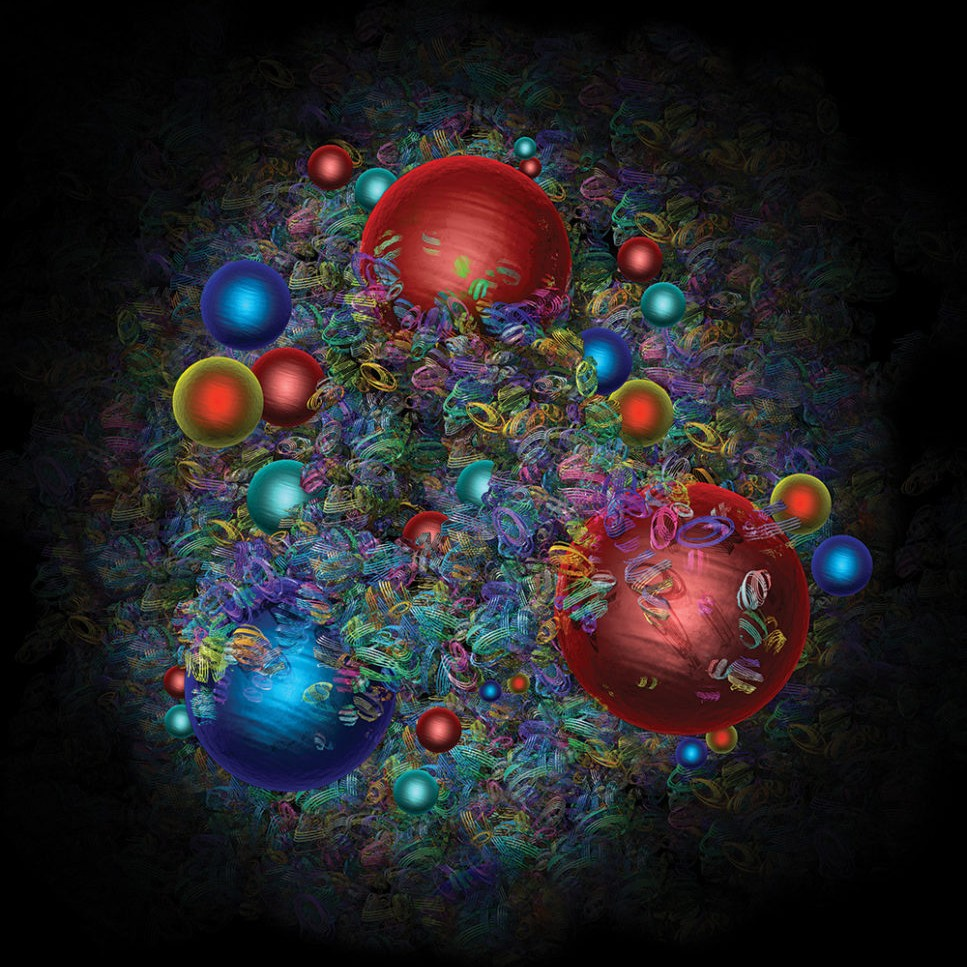
\includegraphics[width=\textwidth]{CERN_Proton.jpg}
        \caption{An artist's representation of a proton\cite{protonImg}.}
        \vspace{0.5\baselineskip}
      \end{figure}
  \end{columns}
\end{frame}

\begin{comment}
\begin{frame}
  \frametitle{Why Lattice Quantum Chromodynamics?}
  \centering
  In quantum field theory scattering amplitudes in the form
  \begin{equation*}
    \bra{f}\ket{i} = \int_{\phi_i}^{\phi_f}\mathcal{D}\prs{\phi} e^{-S[\phi]}
  \end{equation*}
  need to be evaluated.
\onslide<2->
  There are two possible approaches:
  \vspace{\baselineskip}
  \begin{columns}[t]
    \column{0.5\textwidth}
    \centering
    Perturbative\\
    \vspace{\baselineskip}
    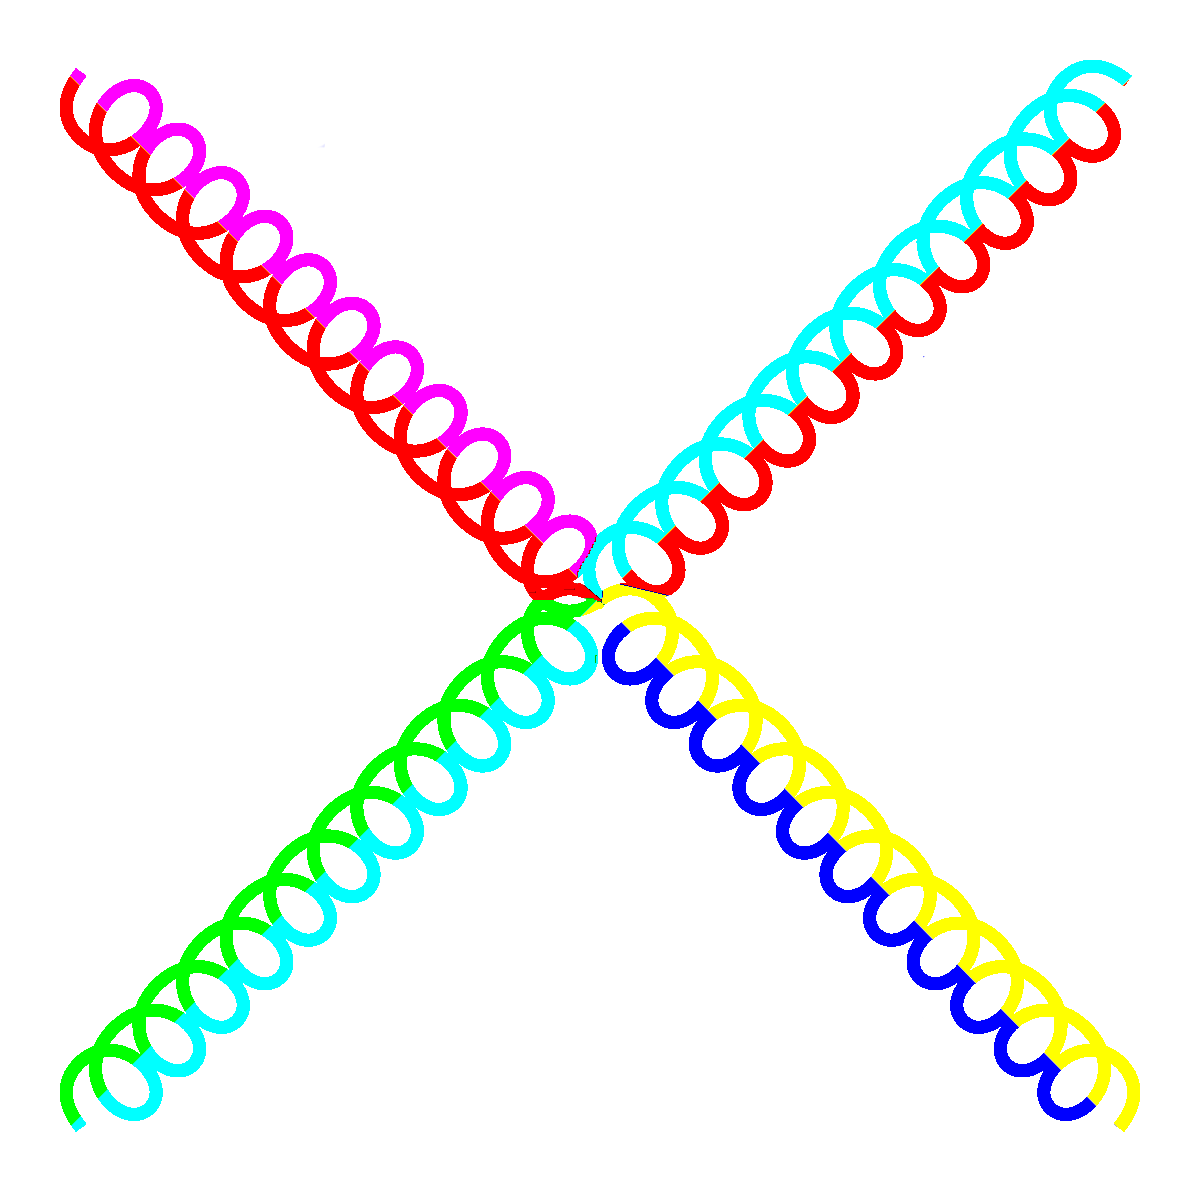
\includegraphics[width=0.4\textwidth]{gluonfd.png}
    \column{0.5\textwidth}
\onslide<3->
    \centering
    Non-Perturbative\\
    \vspace{\baselineskip}
    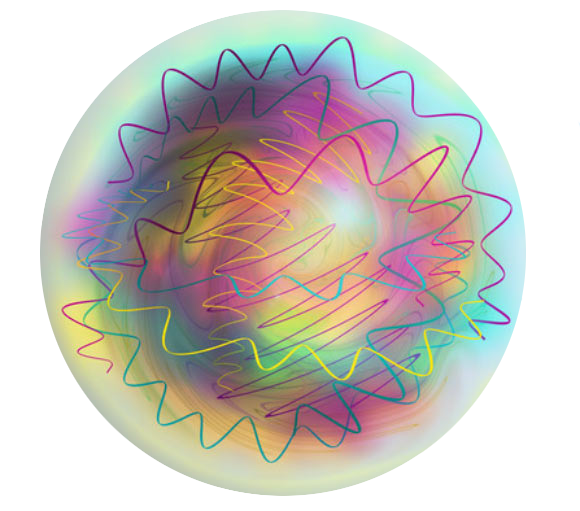
\includegraphics[width=0.45\textwidth]{Glueball.png}
  \end{columns}
\end{frame}

\begin{frame}
  \frametitle{Perturbative vs Non-Perturbative}
  \centering
  \begin{columns}[t]
    \column{0.5\textwidth}
    \centering
\onslide<1->
    Perturbative\\
    \vspace{0.5\baselineskip}
    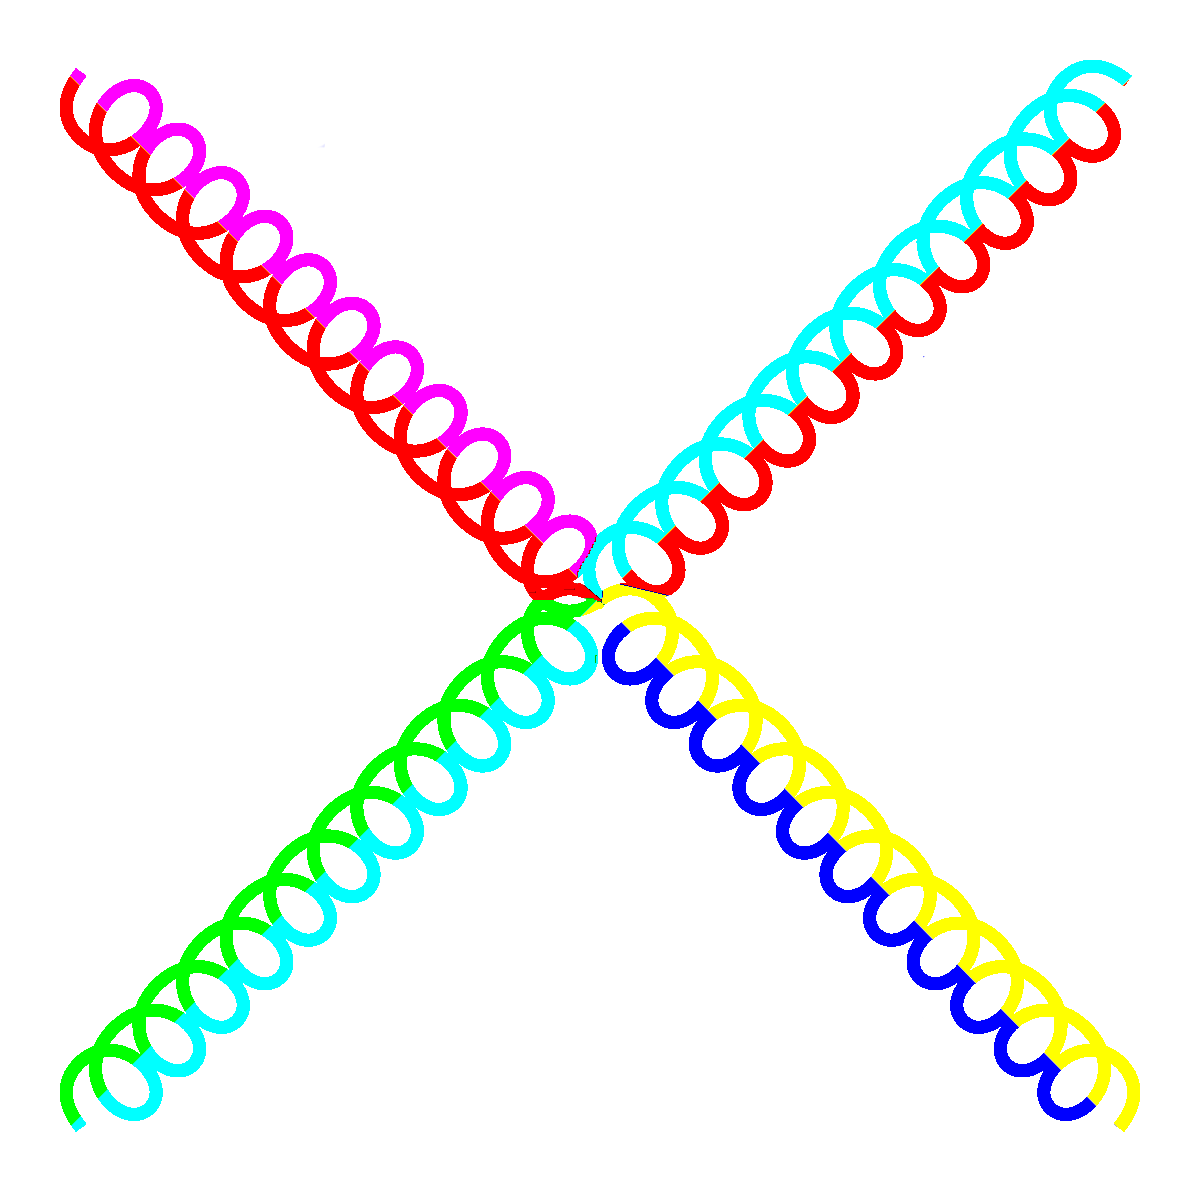
\includegraphics[height=0.4\textwidth]{gluonfd.png}\\
    \vspace{0.5\baselineskip}
    \begin{itemize}
     \item Straightforward series expansion in powers of small $g$ $\Leftrightarrow$ Feynman diagrams with $n$ loops
\onslide<2->
     \item UV divergencies need to be eliminated
\onslide<3->
     \item Fails predicting quantities with essential singularities as $g\rightarrow0$
    \end{itemize}
    \column{0.5\textwidth}
    \centering
\onslide<1->
    Non-Perturbative\\
    \vspace{0.5\baselineskip}
    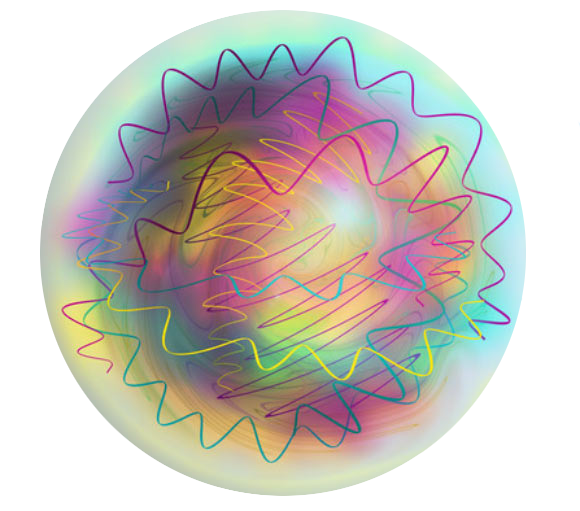
\includegraphics[height=0.4\textwidth]{Glueball.png}\\
    \vspace{0.5\baselineskip}
    \begin{itemize}
\onslide<4->
     \item No straightforward approach
\onslide<5->
     \item Can have a natural cut-off for high momenta $\Rightarrow$ No UV divergencies
\onslide<6->
     \item Can predict quantities with essential singularities as $g\rightarrow0$
    \end{itemize}
  \end{columns}
\end{frame}
\end{comment}

\begin{frame}
  \frametitle{What is a Lattice?}
  \centering
  \begin{columns}
  \column{0.5\textwidth}
\onslide<1->
    \begin{block}{Definition: Lattice $\Lambda$}
      $\Lambda =\left\{\left.\sum _{i=1}^{n}a_{i}e_{i}\;\right\vert \;a_{i}\in \mathbb {Z} \right\}$, with $\prc{e_i}$ any basis of $\R^n$
    \end{block}
    \vspace{5\baselineskip}
\onslide<2->
    \begin{exampleblock}{Hypercubic lattice}
      $\prc{e_i}$ is the canonical basis of $\R^n$\\
      $a$ is called \emph{lattice spacing}.
    \end{exampleblock}
    \vspace{2\baselineskip}
  
  \column{0.1\textwidth}
  
  \column{0.4\textwidth}
\onslide<1->
    \centering
    \begin{figure}
      \includegraphics<1->[width=\textwidth]{two-dimensional-lattice.png}
      \caption{A bidimensional lattice.}
    \end{figure}
\onslide<2->
    \begin{figure}
      \includegraphics<1->[width=0.5\textwidth]{square-lattice.png}
      \caption{A square lattice.}
    \end{figure}
  \end{columns}
\end{frame}

\begin{frame}
  \frametitle{Lattice Field Theory}
  \centering
  \begin{columns}
  \column{0.59\textwidth}
\onslide<1->
    \begin{exampleblock}{Basic idea}
      Fields can take values only in given parts of the lattice, $x\rightarrow n\in\Lambda$.
    \end{exampleblock}
    \vspace{\baselineskip}
\onslide<2->
    Examples:
    \begin{itemize}
      \item \textcolor{blue}{Scalar fields} $\Phi(x)\rightarrow\Phi(n)$ on sites
\onslide<3->
      \item \textcolor{red}{Vector fields} $U_\mu(x)\rightarrow U_\mu(n)$ on links
\onslide<4->
      \item Object with $k$ indices on $k$-symplexes
    \end{itemize}
\onslide<5->
    \vspace{\baselineskip}
    \begin{alertblock}{Beware!}
      Spinorial fields are trickier to be discretized.
    \end{alertblock}
  
  \column{0.01\textwidth}
  
  \column{0.4\textwidth}
    \centering
\onslide<3->
    \begin{block}{Parallel Transporter}
      $U_\mu(x)=\exp(i g a A_\mu(x))$
    \end{block}
\onslide<1->
    \begin{figure}
      \includegraphics<1>[width=0.9\textwidth]{Lattice.png}
      \includegraphics<2>[width=0.9\textwidth]{LatticeScalar.png}
      \includegraphics<3->[width=0.9\textwidth]{LatticeGauge.png}\\
      \caption{A (hyper)cubic lattice in $\R^3$.}
    \end{figure}
  \end{columns}
\end{frame}

\begin{frame}
  \frametitle{Gauge-Invariant Observables and Wilson Action}
  \centering
  \vspace{0.5\baselineskip}
  \begin{columns}
  \column{0.52\textwidth}
\onslide<1->
    The Yang-Mills continuum action is $S_E=\frac14\dV F^{a\mu\nu}(x)F_{\mu\nu}^a(x)$.
\onslide<2->
    \begin{exampleblock}{Definition: Plaquette $U_{\mu\nu}(n)$}
      $U_\mu(n)U_\nu(n+\mu)U^\dagger_\mu(n+\nu)U^\dagger_\nu(n)$
    \end{exampleblock}
    
  \column{0.01\textwidth}
  \column{0.47\textwidth}
\onslide<1->
    On the lattice, every closed path is gauge-invariant.
\onslide<3->
    \begin{block}{Wilson's Idea}
      $S=\frac{\beta}{2N}\sum_{n,\mu,\nu}\mathfrak{Re}\Tr\pr{\id-U_{\mu\nu}(n)}$
    \end{block}
  \end{columns}
\onslide<1->
  \begin{figure}
    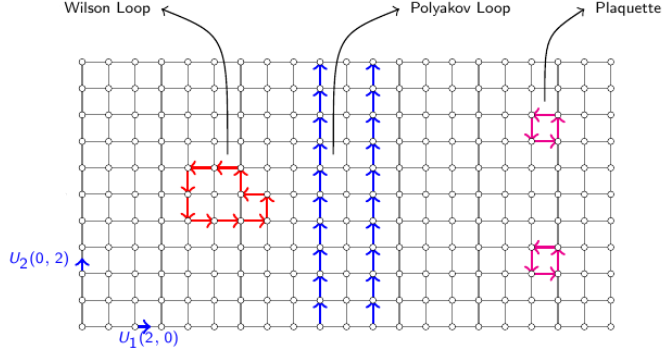
\includegraphics[height=0.4\textheight]{wilsonLoop.png}
    \caption{Gauge-invariant paths on a bidimensional lattice\cite{SigdelDibakar2016}.}
  \end{figure}
\end{frame}

\begin{frame}
  \frametitle{Polyakov Loops and Potential}
  \centering
  \vspace{0.5\baselineskip}
  \begin{columns}
  \column{0.52\textwidth}
\onslide<1->
    If the time coordinate is taken to be periodic, more closed paths arise.
    \begin{block}{Polyakov Loop}
      $P(n)=\Tr\prod_{t=0}^{T-1} U_t(n)$
    \end{block}
  
  \column{0.01\textwidth}
  \column{0.47\textwidth}
\onslide<2->
    The expectation value of two Polyakov loops is the potential.
    \begin{exampleblock}{Potential}
      $V(R)=-\frac1T\log<P(0)P^\dagger(R)>$
    \end{exampleblock}
  \end{columns}
  \vspace{0.25\baselineskip}

\onslide<1->
  \begin{figure}
    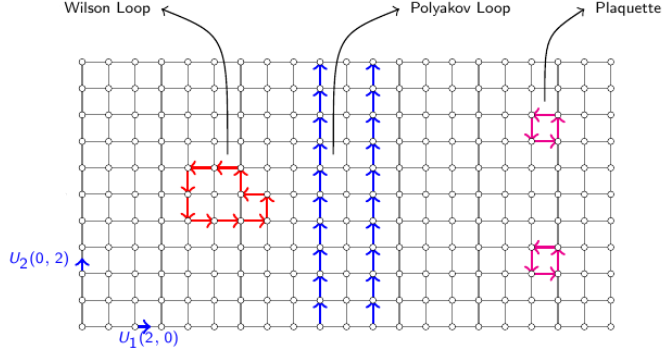
\includegraphics[height=0.4\textheight]{wilsonLoop.png}
    \caption{Gauge-invariant paths on a bidimensional lattice\cite{SigdelDibakar2016}.}
  \end{figure}
\end{frame}

\begin{frame}
  \frametitle{Monte Carlo Simulations}
  \centering
  Computers are used to simulate Lattice Field Theories
  \vspace{.5\baselineskip}
  \begin{itemize}
    \item<2-> Random configurations of link variables are generated.
    \item<3-> Proper Monte Carlo algorithms evolve the configurations towards minimums of the action.
    \item<4-> A great number of observables is evaluated and then their mean value is computed.
  \end{itemize}
  \vspace{.5\baselineskip}
  \begin{figure}[b]
    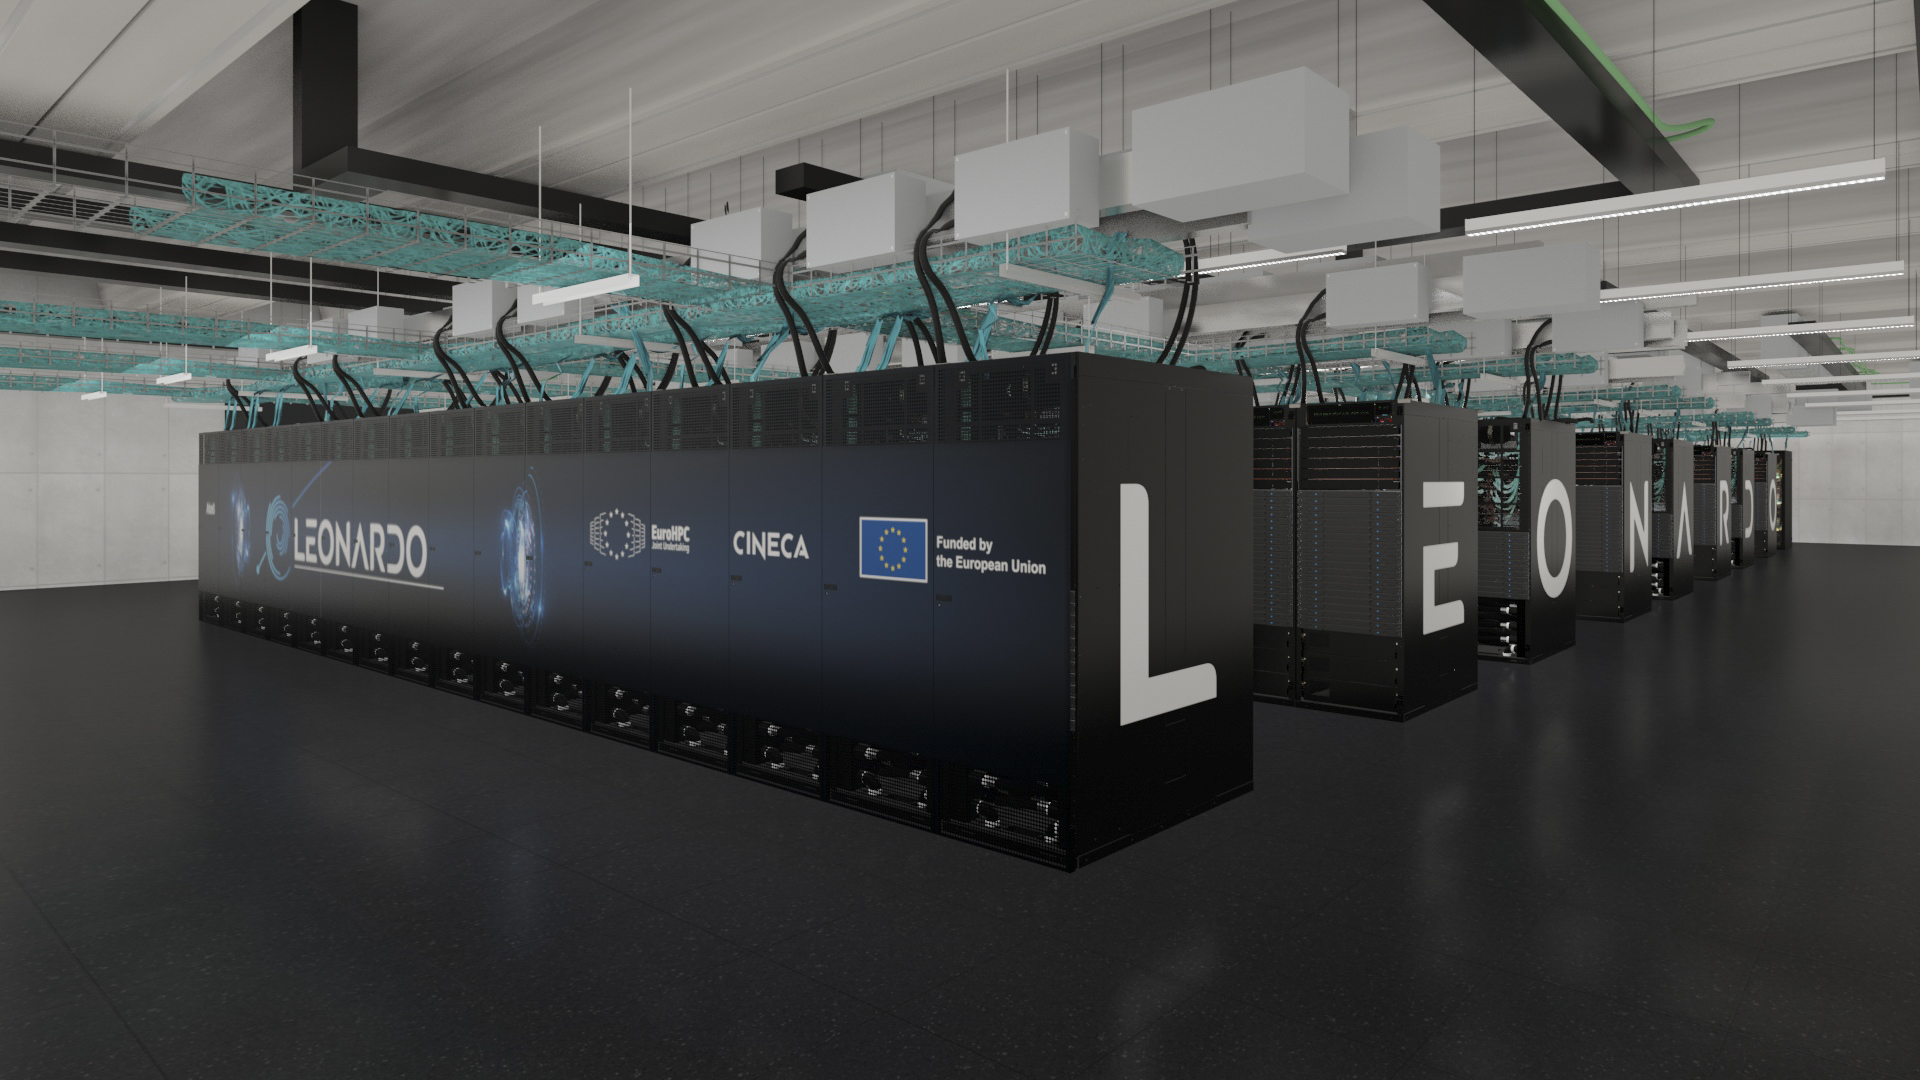
\includegraphics[width=.7\textwidth]{Leonardo.jpg}
    \caption{A rendering of the CINECA Leonardo supercomputer\cite{LeonardoImg}.}
  \end{figure}
\end{frame}

\begin{frame}
  \frametitle{Lattice Symmetries}
  \centering
\onslide<1->
  Poincaré Group can be divided in:
  \begin{columns}[t]
  \column{0.45\textwidth}
    \centering
    \begin{exampleblock}{\centering Translations}
      \vspace{-\baselineskip}
\onslide<2->
      \begin{align*}
        x^\mu \rightarrow& x^\mu+\varepsilon^\mu \\
        &\Downarrow \\
        n \rightarrow& n+a\hat\mu
      \end{align*}
    \end{exampleblock}
    \vspace{2.5\baselineskip}
\onslide<4->
    $a\hat\mu \rightarrow \varepsilon^\mu$ for $a\rightarrow0$
  
  \column{0.1\textwidth}
  \column{0.45\textwidth}
    \centering
\onslide<1->
    \begin{exampleblock}{\centering Rotations}
      \vspace{-\baselineskip}
\onslide<3->
      \begin{align*}
        x^\mu \rightarrow R^\mu_\nu x^\nu &\quad R\in \mathit{SO}(4) \\
        &\Downarrow \\
        n \rightarrow \Gamma n &\quad \Gamma\in G_{\Lambda_{SH}}
      \end{align*}
    \end{exampleblock}
    $G_{\Lambda_{SH}}$: group of rotations of multiples of $90\degree$ around any axis.\\
    \vspace{0.6\baselineskip}
\onslide<5->
    $\Gamma \xcancel{\rightarrow}R$ for $a\rightarrow0$
  \end{columns}
  \vspace{\baselineskip}
  \begin{columns}
\onslide<6->
  \column{0.6\textwidth}
    \begin{alertblock}{Important:}
      Rotational invariance seems to be broken.
    \end{alertblock}
  \end{columns}
\end{frame}

\begin{frame}
  \frametitle{Rotational Invariance Restoration - Lang and Rebbi}
  Equipotential surfaces become spheres as the continuum limit is approached\cite{Lang:1982tj}.\\
  The gauge group used was the discrete icosahedral subgroup $\tilde{Y}\subset\mathit{SU}(2)$.
  \begin{figure}
    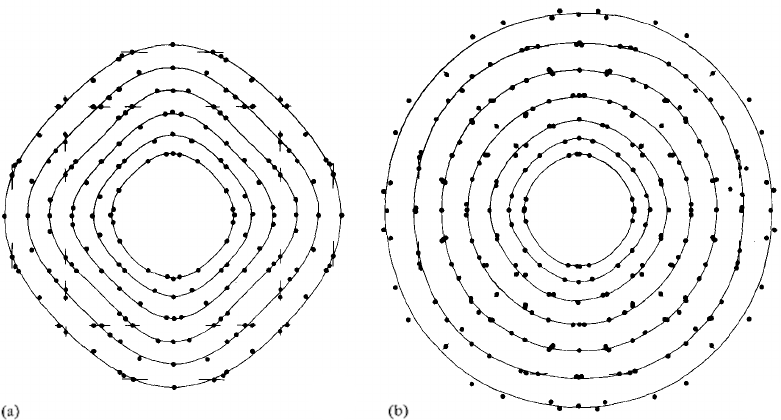
\includegraphics[width=.74\textwidth]{LangRebbi.png}
    \caption{Restoration of rotational invariance from (a) $\beta=2$, $n_s=8$, $n_t=4$ to (b) $\beta=2.25$, $n_s=16$, $n_t=6$; the curves represent equipotential curves.}
  \end{figure}
\end{frame}

\begin{frame}
  \frametitle{Rotational Invariance Restoration}
  Results of simulations for gauge group $\mathit{SU}(2)$ with $20000$ measurements each\footnote{The simulation code is based on the code presented in refs.~\mycite{Panero:2009tv,Mykkanen:2012ri}.}.
  Approach slightly different than Lang and Rebbi's.
%  because $a(\beta)\approx\Lambda e^{-b_0\beta}$, with $\Lambda$, $b_0>0$
  \vspace{-0.5\baselineskip}
  \begin{columns}
  \column{0.4\textwidth}
    \begin{figure}
      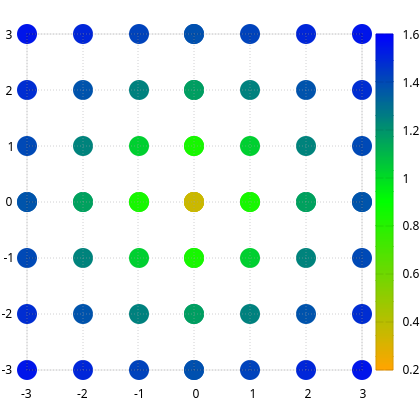
\includegraphics[width=\textwidth]{plots/RotSymm_nt4_ns8_beta2.20.png}
      \caption{Potential from $\beta=2.20$, $n_s=8$, $n_t=4$.}
    \end{figure}
  \column{0.4\textwidth}
    \begin{figure}
      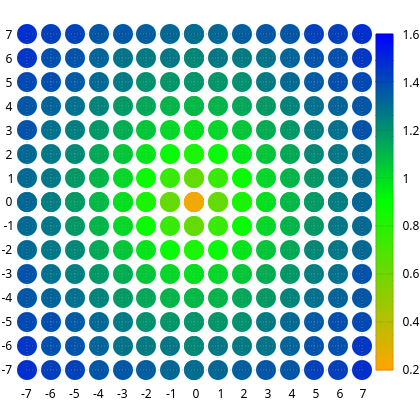
\includegraphics[width=\textwidth]{plots/RotSymm_nt6_ns16_beta2.35.png}
      \caption{Potential from $\beta=2.35$, $n_s=16$, $n_t=6$.}
    \end{figure}
  \end{columns}
\end{frame}

\begin{frame}
  \frametitle{Higher Symmetry Lattices}
\onslide<1->
  Other, more rotational-symmetric, lattices have been used:\\
  \begin{columns}
    \column{0.47\textwidth}
\onslide<1->
    \centering
      \begin{block}{\centering
        Body Centered Tesseract
        }
        \begin{itemize}
          \item $24$ nearest neighbours
          \item $1152$-element symmetry group
        \end{itemize}
      \end{block}
      \begin{figure}
        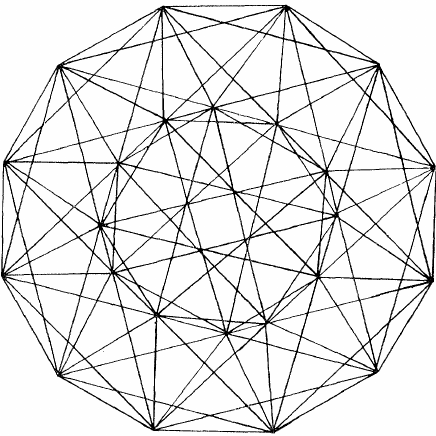
\includegraphics[width=0.55\textwidth]{Tesseract.png}
        \caption{Two-dimensional projection of a BCT\cite{Celmaster:1982ht}.}
      \end{figure}
    
    \column{0.02\textwidth}
    \column{0.47\textwidth}
\onslide<2->
    \centering
      \begin{block}{\centering
          $F_4$ coroots lattice\cite{Neuberger:1987kt}
          }
          \begin{itemize}
            \item $48$ nearest neighbours
            \item $2304$-element symmetry group
          \end{itemize}
        \end{block}
      \begin{figure}
        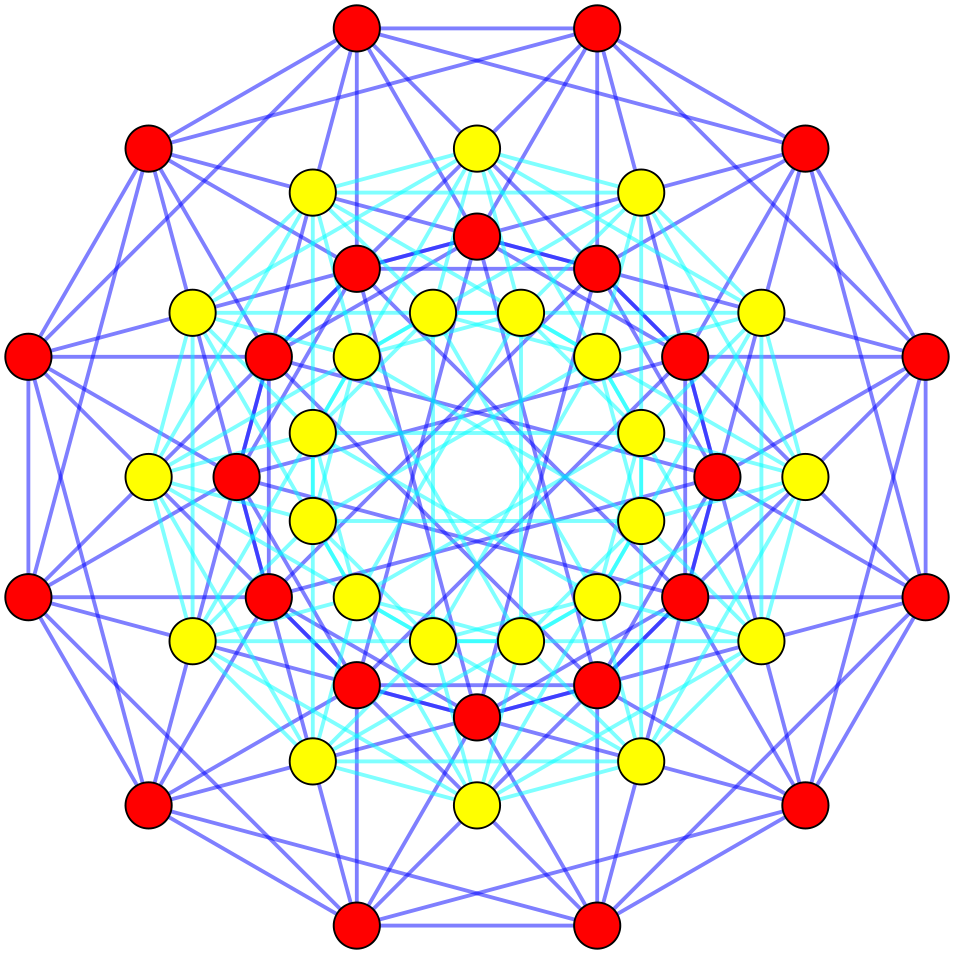
\includegraphics[width=0.55\textwidth]{F4_root_lattice.png}
        \caption{Two-dimensional projection of a $F_4$ coroots lattice\cite{f4image}.}
      \end{figure}
  \end{columns}
\onslide<1->
  \footnotesize
  The SH lattice has $8$ nearest neighbours and a $384$-element symmetry group.
\end{frame}

\begin{frame}
  \frametitle{Body Centered Tesseract (BCT)}
  \centering
  \begin{columns}
  \column{0.6\textwidth}
    \begin{itemize}
      \item<1->[\ding{228}] Obtained from Simple Hypercubic lattice considering also the centers;
      \item<2->[\ding{228}] Elementary cell is the $24$-cell;
      \item<3->[\ding{228}] Has $24$ nearest neighbours:
      \begin{itemize}
        \item<3-> The $8$ possible permutations of $\pr{\pm1,0,0,0}$
        \item<3-> The $16$ vectors of the form $\pr{\pm\frac12,\pm\frac12,\pm\frac12,\pm\frac12}$
      \end{itemize}
      \vspace{0.25\baselineskip}
      \item<4->[\ding{228}] Plaquettes are triangular;
      \item<5->[\ding{228}] Contains the Simple Hypercubic lattice;
      \item<6->[\ding{228}] Has been used to simulate $\mathit{SU}(2)$ Yang-Mills theories,\\in \mycite{Celmaster:1982ht}.
    \end{itemize}

  \column{0.4\textwidth}
  \centering
\onslide<1->
    \begin{figure}
      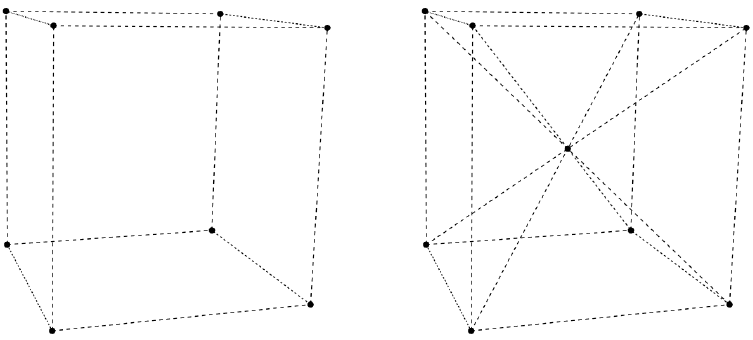
\includegraphics[width=\textwidth]{CellsCrop.png}
      \caption{Cubic Cell (left) and BC Cubic Cell (right).}
    \end{figure}
    \vspace{-\baselineskip}
\onslide<2->
    \begin{figure}
      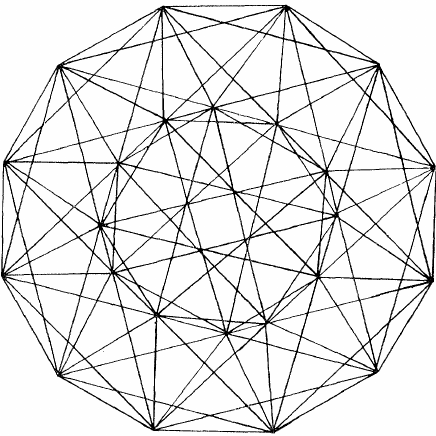
\includegraphics[width=.5\textwidth]{Tesseract.png}
      \caption{Bidimensional projection of the $24$-cell.}
    \end{figure}
  \end{columns}
\end{frame}

\begin{frame}
  \frametitle{$F_4$ Coroots Lattice}
  \centering
  \begin{columns}
  \column{0.6\textwidth}
    \begin{itemize}
      \item<1->[\ding{228}] Obtained from the roots lattice of the exceptional Lie algebra $F_4$ and its dual;
      \item<2->[\ding{228}] Has $48$ nearest neighbours:
      \begin{itemize}
        \item The $24$ roots are all possible permutations of coordinate positions of $\pr{\pm1,\pm1,0,0}$
        \vspace{0.25\baselineskip}
        \item<3-> The $24$ dual roots (coroots) are:
        \begin{itemize}
          \item<3->[\ding{109}] The $8$ possible permutations of $\pr{\pm1,0,0,0}$
          \item<3->[\ding{109}] The $16$ vectors of the form $\pr{\pm\frac12,\pm\frac12,\pm\frac12,\pm\frac12}$
        \end{itemize}
      \end{itemize}
      \item<4->[\ding{228}] Exists only in $4$ dimensions;
      \item<5->[\ding{228}] Is a more symmetric version of the BCT;
      \item<6->[\ding{228}] Has been used only to simulate scalar fields, in \mycite{Neuberger:1987kt}.
    \end{itemize}

  \column{0.4\textwidth}
\onslide<1->
    \begin{figure}
      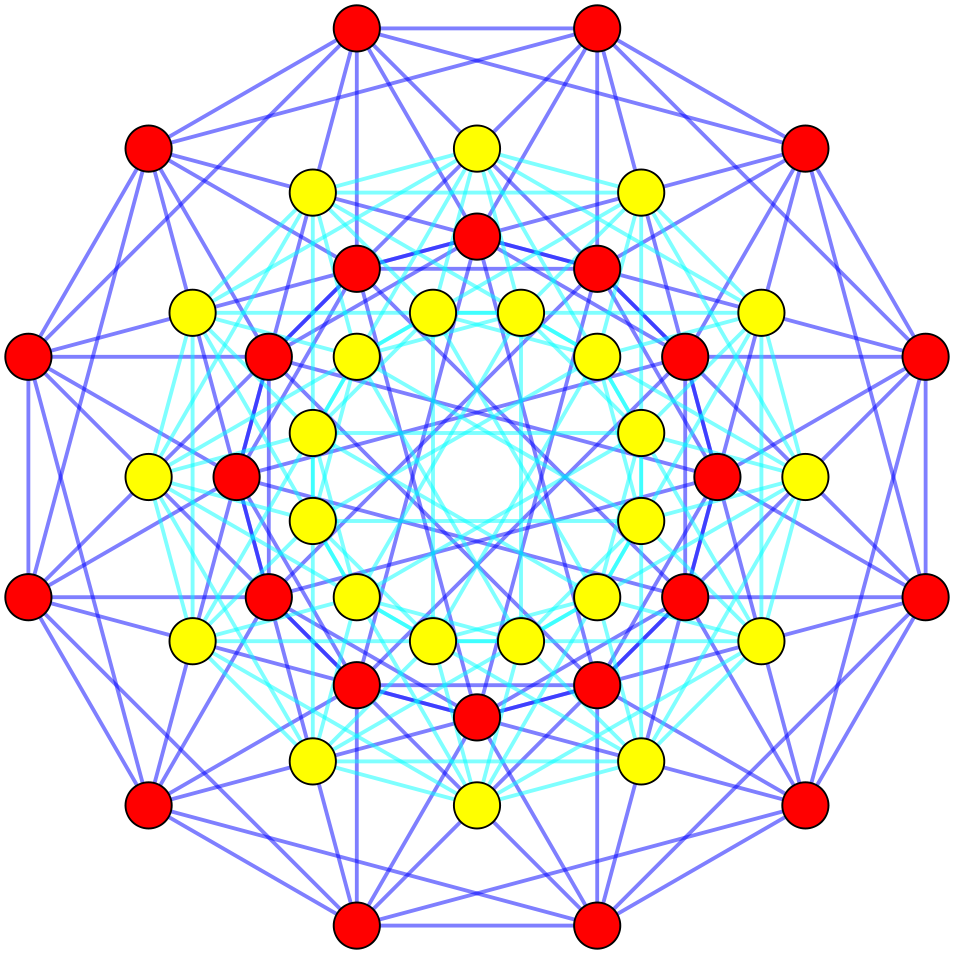
\includegraphics[width=\textwidth]{F4_root_lattice.png}
      \caption{
\only<1>
        {Bidimensional projection of the $F_4$ lattice.\vspace{2\baselineskip}}
\only<2>
        {The $24$ roots (\textcolor{red}{red}) of the $F_4$ lattice, projected on a bidimensional plane.\vspace{\baselineskip}}
\only<3->
        {The $24$ roots (\textcolor{red}{red}) and the $24$ coroots (\textcolor{yellow}{yellow}) of the $F_4$ lattice, projected on a bidimensional plane.}
      }
    \end{figure}
  \end{columns}
\end{frame}

\begin{frame}
  \frametitle{Simulations on SH Lattice}
  \centering
  \begin{columns}[c]
    \column{.52\textwidth}
    \centering
    Wilson Action:
    \begin{equation*}
      S_W = \frac\beta{2N}\sum_{x\in\Lambda}\sum_{\mu<\nu}\mathfrak{Re}\Tr[\id-U_{\mu\nu}(x)]
    \end{equation*}
    Plaquette:
    \begin{equation*}
      U_{\mu\nu} = \textcolor<2->{red}{U_\mu(x)}\textcolor<2->{blue}{U_\nu(x+\hat\mu)U^\dagger_\mu(x+\hat\nu)U^\dagger_\nu(x)}
    \end{equation*}
  
    \column{.48\textwidth}
    \centering
\onslide<1->
    \begin{figure}[!htbp]
      \centering
      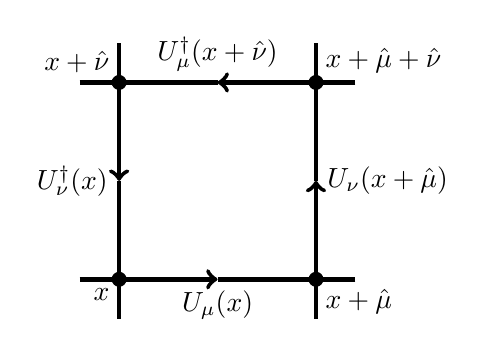
\begin{tikzpicture}
        \filldraw[black] (0,0) circle (2.5pt) node[anchor=north east]{$x$};
        \filldraw[black] (0,2.5) circle (2.5pt) node[anchor=south east]{$x+\hat\nu$};
        \filldraw[black] (2.5,0) circle (2.5pt) node[anchor=north west]{$x+\hat\mu$};
        \filldraw[black] (2.5,2.5) circle (2.5pt) node[anchor=south west]{$x+\hat\mu+\hat\nu$};
        \draw[ultra thick] (-0.5,0) -- (0,0);
        \draw[ultra thick] (0,-0.5) -- (0,0);
        \draw[ultra thick,->] (0,0) -- (1.25,0) node[anchor=north]{$U_\mu(x)$};
        \draw[ultra thick   ] (1.25,0) -- (2.5,0);
        \draw[ultra thick]  (3,0) -- (2.5,0);
        \draw[ultra thick] (2.5,-0.5) -- (2.5,0);
        \draw[ultra thick,->] (2.5,0) -- (2.5,1.25) node[anchor=west]{$U_\nu(x+\hat\mu)$};
        \draw[ultra thick   ] (2.5,1.25) -- (2.5,2.5);
        \draw[ultra thick]  (3,2.5) -- (2.5,2.5);
        \draw[ultra thick]  (2.5,3) -- (2.5,2.5);
        \draw[ultra thick,->] (2.5,2.5) -- (1.25,2.5) node[anchor=south]{$U^\dagger_\mu(x+\hat\nu)$};
        \draw[ultra thick   ] (1.25,2.5) -- (0,2.5);
        \draw[ultra thick] (-0.5,2.5) -- (0,2.5);
        \draw[ultra thick]  (0,3) -- (0,2.5);
        \draw[ultra thick,->] (0,2.5) -- (0,1.25) node[anchor=east]{$U^\dagger_\nu(x)$};
        \draw[ultra thick   ] (0,1.25) -- (0,0);
      \end{tikzpicture}
    \end{figure}
  \end{columns}
\onslide<2->
  \begin{columns}[c]
    \column{.35\textwidth}
    \centering
    \raggedleft
    \tikz[baseline]{
      \node[fill=green!20, ellipse, anchor=base] (atoms)
      {$6$ staples for each link};
    }
    
    \column{.65\textwidth}
    \centering
    \begin{figure}[!htbp]
      \centering
      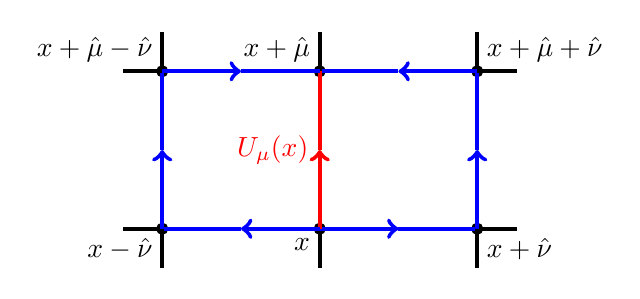
\begin{tikzpicture}
        \filldraw[black]  (0,0) circle (2pt) node[anchor=north east]{$x$};
        \filldraw[black]  (0,2) circle (2pt) node[anchor=south east]{$x+\hat\mu$};
        \filldraw[black]  (2,0) circle (2pt) node[anchor=north west]{$x+\hat\nu$};
        \filldraw[black]  (2,2) circle (2pt) node[anchor=south west]{$x+\hat\mu+\hat\nu$};
        \filldraw[black] (-2,0) circle (2pt) node[anchor=north east]{$x-\hat\nu$};
        \filldraw[black] (-2,2) circle (2pt) node[anchor=south east]{$x+\hat\mu-\hat\nu$};
        \draw[ultra thick] (0,-0.5) -- (0,0);
        \draw[color=blue,ultra thick,->] (0,0) -- (1,0);
        \draw[color=blue,ultra thick   ] (1,0) -- (2,0);
        \draw[ultra thick]  (2.5,0) -- (2,0);
        \draw[ultra thick] (2,-0.5) -- (2,0);
        \draw[color=blue,ultra thick,->] (2,0) -- (2,1);
        %node[anchor=west]{$P^\dagger_i(x)$};
        \draw[color=blue,ultra thick   ] (2,1) -- (2,2);
        \draw[ultra thick]  (2.5,2) -- (2,2);
        \draw[ultra thick]  (2,2.5) -- (2,2);
        \draw[color=blue,ultra thick,->] (2,2) -- (1,2);
        \draw[color=blue,ultra thick   ] (1,2) -- (0,2);
        \draw[ultra thick]  (0,2.5) -- (0,2);
        \draw[color=red,ultra thick,->] (0,0) -- (0,1) node[anchor=east]{$U_\mu(x)$};
        \draw[color=red,ultra thick   ] (0,1) -- (0,2);
        
        \draw[color=blue,ultra thick,->] (0,0) -- (-1,0);
        \draw[color=blue,ultra thick   ] (-1,0) -- (-2,0);
        \draw[ultra thick]  (-2.5,0) -- (-2,0);
        \draw[ultra thick] (-2,-0.5) -- (-2,0);
        \draw[color=blue,ultra thick,->] (-2,0) -- (-2,1);
        %node[anchor=east]{$P^\dagger_j(x)$};
        \draw[color=blue,ultra thick   ] (-2,1) -- (-2,2);
        \draw[ultra thick]  (-2.5,2) -- (-2,2);
        \draw[ultra thick]  (-2,2.5) -- (-2,2);
        \draw[color=blue,ultra thick,->] (-2,2) -- (-1,2);
        \draw[color=blue,ultra thick   ] (-1,2) -- (-0,2);
      \end{tikzpicture}
  %    \caption{Example of a link (\textcolor{red}{red}) with two of its staples (\textcolor{blue}{blue}).}
    \end{figure}
  \end{columns}
\end{frame}

\begin{frame}
  \frametitle{Simulations on BCT Lattice}
  \centering\begin{columns}[c]
    \column{.52\textwidth}
    \centering
    BCT Action:
    \begin{equation*}
      S_{BCT} = \frac\beta8 \sum_\bigtriangleup \mathfrak{Re}\Tr \Utriang
    \end{equation*}
    Plaquette:
    \begin{equation*}
      \Utriang = \textcolor<2->{red}{U_v(x)}\textcolor<2->{blue}{U_w(x+\hat{v})U^\dagger_{v+w}(x)}
    \end{equation*}
  
    \column{.48\textwidth}
    \centering
\onslide<1->
    \begin{figure}[!htbp]
      \centering
      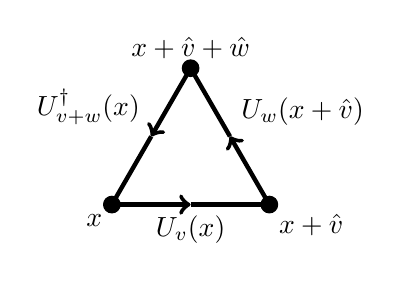
\begin{tikzpicture}
        \filldraw[black]  (0,0) circle (3pt) node[anchor=north east]{$x$};
        \filldraw[black]  (2,0) circle (3pt) node[anchor=north west]{$x+\hat{v}$};
        \filldraw[black]  (1,1.732) circle (3pt) node[anchor=south]{$x+\hat{v}+\hat{w}$};
        \draw[ultra thick,->] (0,0) -- (1,0) node[anchor=north]{$U_v(x)$};
        \draw[ultra thick   ] (1,0) -- (2,0);
        \draw[ultra thick,->] (2,0) -- (1.5,0.866) node[anchor=south west]{$U_w(x+\hat{v})$};
        \draw[ultra thick   ] (1.5,0.866) -- (1,1.732);
        \draw[ultra thick,->] (1,1.732) -- (0.5,0.866) node[anchor=south east]{$U^\dagger_{v+w}(x)$};
        \draw[ultra thick   ] (0.5,0.866) -- (0,0);
      \end{tikzpicture}
    \end{figure}
  \end{columns}
  \vspace{1.5\baselineskip}
  
\onslide<2->
  \begin{columns}[c]
    \column{.05\textwidth}
    \column{.3\textwidth}
    \centering
    \tikz[baseline]{
      \node[fill=green!20, ellipse, anchor=base] (atoms)
      {$8$ staples for each link};
    }
    \column{.05\textwidth}
    
    \column{.6\textwidth}
    \centering
    \begin{figure}[!htbp]
      \centering
      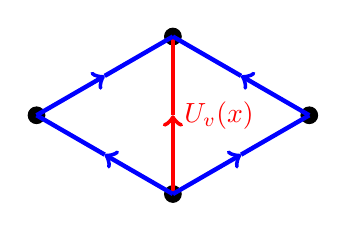
\begin{tikzpicture}
        \filldraw[black]  (0,0) circle (3pt);
        \filldraw[black]  (0,2) circle (3pt);
        \filldraw[black]  (2.598*2/3,1) circle (3pt);
        \filldraw[black]  (-2.598*2/3,1) circle (3pt);
        \draw[red, ultra thick,->] (0,0) -- (0,1) node[anchor=west]{$U_v(x)$};
        \draw[red, ultra thick   ] (0,1) -- (0,2);
        
        \draw[blue, ultra thick,->] (0,0) -- (2.598/3,1.5/3);
        %node[text=black, anchor=north west]{$w$};
        \draw[blue, ultra thick   ] (2.598/3,1.5/3) -- (2.598*2/3,1);
        \draw[blue, ultra thick,->] (2.598*2/3,1) -- (2.598/3,1.5*2/3+1.5/3);
        %node[text=black, anchor=south west]{$u$};
        \draw[blue, ultra thick   ] (2.598/3,1.5*2/3+1.5/3) -- (0,2);
        
        \draw[blue, ultra thick,->] (0,0) -- (-2.598/3,1.5/3);
        %node[text=black, anchor=north east]{$u$};
        \draw[blue, ultra thick   ] (-2.598/3,1.5/3) -- (-2.598*2/3,1.5*2/3);
        \draw[blue, ultra thick,->] (-2.598*2/3,1) -- (-2.598/3,1.5*2/3+1.5/3);
        %node[text=black, anchor=south east]{$w$};
        \draw[blue, ultra thick   ] (-2.598/3,1.5*2/3+1.5/3) -- (0,2);
      \end{tikzpicture}
    \end{figure}
  \end{columns}
\end{frame}

\begin{frame}
  \frametitle{Simulation Results}
  \centering
  Average Plaquette as a function of Computer Time
  \begin{columns}[c]
    \column{.5\textwidth}
      \begin{figure}
        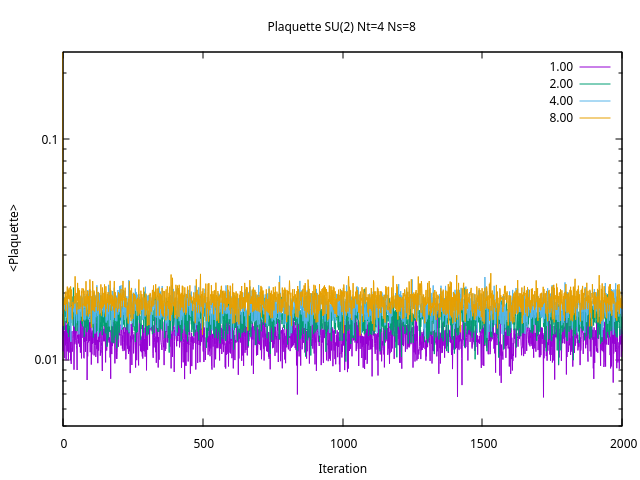
\includegraphics[width=\textwidth]{plaquetteSmallBCT.png}
        \caption{Lattice with $n_t=4$, $n_s=8$.}
      \end{figure}
    
    \column{.5\textwidth}
      \begin{figure}
        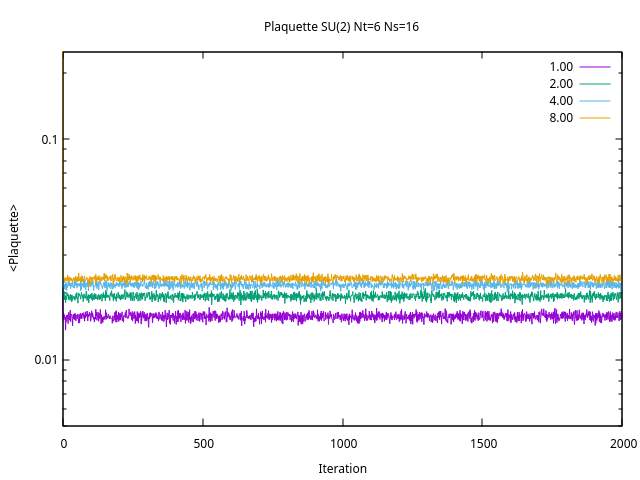
\includegraphics[width=\textwidth]{plaquetteBigBCT.png}
        \caption{Lattice with $n_t=6$, $n_s=16$.}
      \end{figure}
  \end{columns}
\end{frame}

\begin{frame}
  \frametitle{Simulation Results}
  \centering
  Average Plaquette as a function of $\beta$\\
  \vspace{\baselineskip}
  \includegraphics[width=.5\textwidth]{plaquetteBetaBCT.png}\\
  \vspace{\baselineskip}
  Purple data is from a lattice with $n_t=4$, $n_s=8$.\\
  Green data is from a lattice with $n_t=6$, $n_s=16$.
\end{frame}

\begin{frame}
  \frametitle{Conclusions}
  \centering
  \begin{itemize}
    \item<1->[\ding{228}] Several tests of consistency (gauge invariance, plaquette correctness, etc.) have been successfully made;
    \item<2->[\ding{228}] Rapid convergence of the plaquette value has been observed;
    \item<3->[\ding{228}] Plaquette value as a function of $\beta$ do not show expected results:
    \begin{itemize}
      \item<3-> Bigger error bars (w.r.t. SH lattice);
      \item<4-> Different trend than results obtained with different simulations in literature\cite{Celmaster:1983vy};
    \end{itemize}
    \item<5->[\ding{228}] Possible explanation: values of $\beta$ used are far from the continuum limit (assuming there are no bugs in the code);
    \item<6->[\ding{228}] Extension to $F_4$ lattice would add "improvement terms" and more symmetries;
    \item<7->[\ding{228}] Rotational invariance studies could be made.
  \end{itemize}
\end{frame}

\begin{comment}
\begin{frame}
  \frametitle{Work in Progress}
  \begin{columns}
  \column{0.5\textwidth}
\onslide<1->
    \begin{itemize}
    \item Implement the $F_4$ lattice in the simulation program and make efficiency studies;
    \vspace{5\baselineskip}
\onslide<2->
    \item Make a rotational invariance study on the new lattice, hoping to get better results than the Simple Hypercubic lattice.
    \end{itemize}
    
\onslide<1->
  \column{0.1\textwidth}
  \column{0.3\textwidth}
    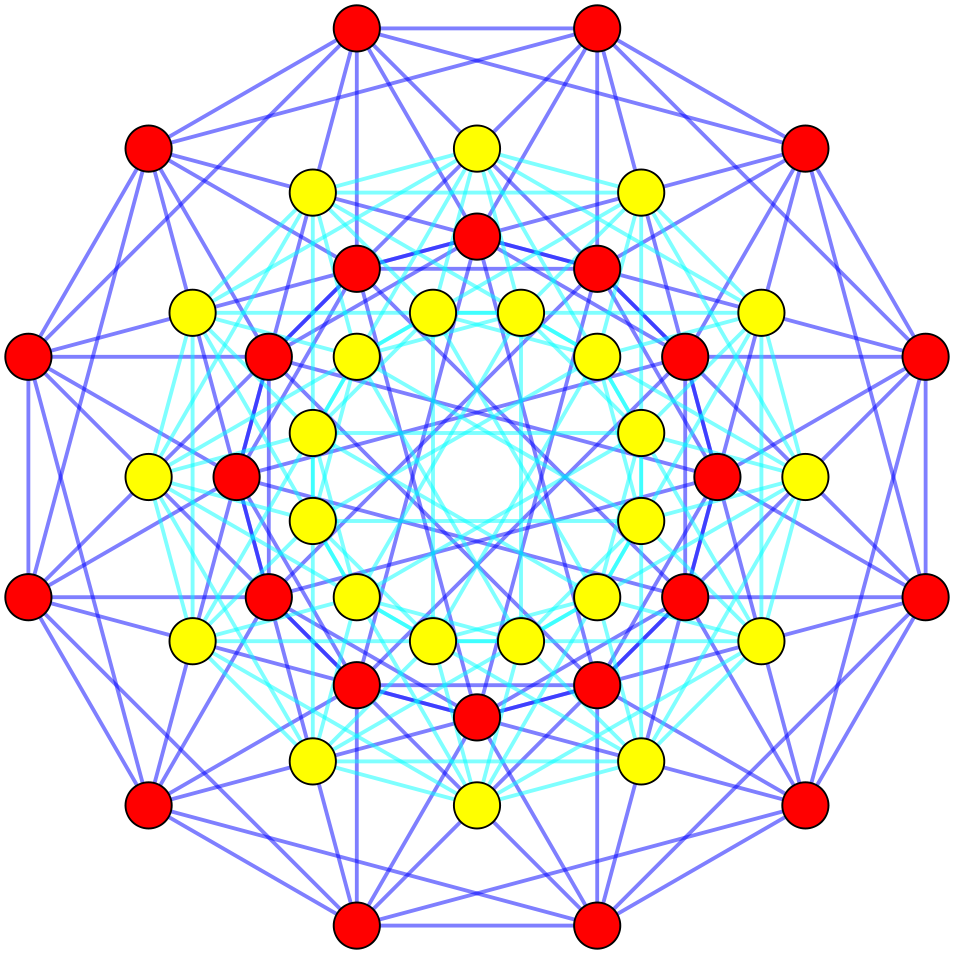
\includegraphics[width=\textwidth]{F4_root_lattice.png}\\
    \vspace{\baselineskip}
\onslide<2->
    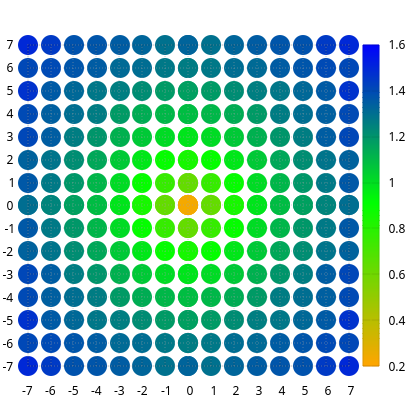
\includegraphics[width=\textwidth]{plots/XY_Plane_nt6_ns16_beta2.35_copied.png}
  \end{columns}
\end{frame}
\end{comment}

\begin{frame}
  \centering
  \Huge
  Thank you for your attention
\end{frame}

\begin{frame}[allowframebreaks]
  \frametitle{Bibliography}
  \printbibliography
\end{frame}

\end{document}
